\subsubsection{Partitions of Unity and the Existence of Bump Functions}\label{sec:partitionsofunity}
\begin{definition}[Topological Space]
    A \textit{topological space} is a pair \((X,\tau)\), where \(X\) is a set and \(\tau\) is a collection of subsets of \(X\) satisfying the following properties:
    \begin{enumerate}
        \item \(\varnothing\in\tau\) and \(X\in\tau\),
        \item The union of any (possibly infinite) collection of sets in \(\tau\) is also in \(\tau\),
        \item The intersection of any finite collection of sets in \(\tau\) is also in \(\tau\).
    \end{enumerate}
    The collection \(\tau\) is called a \textit{topology} on \(X\), and its elements are referred to as \textit{open sets} under the topology \(\tau\).
\end{definition}
Obviously the statement ``let \(X\) be a topological space'' itself has little meaning. However, when the topology is implicitly obvious then it may be verbally elided.

We now provide a formal definition of the connectivity of sets:
\begin{definition}
    A topological space \(X\) is \textit{disconnected} if it can be written as the union of two nonempty disjoint open sets. Otherwise, it is \textit{connected}.
\end{definition}
A topology allows the definition and general conceptualization of continuity, convergence, and connectivity in a general setting, without necessarily relying on a notion of distance (a metric). For example, in a topological space, a function \(f:X\to Y\) between two topological spaces is said to be \emph{continuous} if the preimage of every open set in \(Y\) is an open set in \(X\). This generalizes the familiar \(\varepsilon\)--\(\delta\) definition of continuity.
\begin{example}
    Consider the function \(f:\mathbb{R}\to\mathbb{R}\) defined by
    \[f(x)=
        \begin{dcases}
            1 & \qif* x\ge0, \\
            0 & \qif* x<0.
        \end{dcases}\]
    We equip both the domain and codomain with the standard topology on \(\mathbb{R}\). Let \(V=(0.5,1.5)\subseteq\mathbb{R}\). Then the preimage of \(V\) is
    \[f^{-1}(V)=\cbraces{x\in\mathbb{R}}{f(x)\in(0.5,1.5)}=\mathbb{R}_{\ge0},\]
    which is not an open set in the standard topology on \(\mathbb{R}\). Thus, \(f\) is not continuous.
\end{example}
\begin{definition}[Basis of a Topology]
    For a topological space \((X,\tau)\), a \textit{basis} \(\mathfrak{B}\subseteq\tau\) is a subcollection of \(\tau\) such that every set in \(\tau\) is equal to the union of some subcollection of \(\mathfrak{B}\).
\end{definition}
It is easy to see that \(\mathfrak{B}\) forms an open cover of \(X\). Moreover, for any two sets \(B_1,B_2\in\mathfrak{B}\) and any \(x\in B_1\cap B_2\), there exists \(B_3\in\mathfrak{B}\) such that \(x\in B_3\subseteq B_1\cap B_2\).

In a topological space \(X\), a subset can be open, closed (the complement of some open set), both (clopen), or neither. The only clopen sets that exist in any topological space \(X\) are \(\varnothing\) and \(X\) if \(X\) is connected. A technique used in many proofs in complex analysis relies on the following fact:
\begin{theorem}[Connectivity Argument]\label{thm:connectedtopologicalspaceclopensets}
    A topological space \(X\) is \textit{connected} if and only if \(X\) and \(\varnothing\) are the only clopen subsets of \(X\).
\end{theorem}
\begin{proof}
    Suppose \(X\) is connected and let \(A\subseteq X\) be clopen. Then \(A\) and \(X\setminus A\) are both open in \(X\), disjoint, and their union is \(X\). Thus, either \(A=\varnothing\) or \(X\setminus A=\varnothing\) (i.e., \(A=X\)).

    Conversely, suppose \(X\) is disconnected. Then there exist nonempty open sets \(U,V\subseteq X\) such that \(U\cap V=\varnothing\) and \(U\cup V=X\). Thus, \(U=X\setminus V\) and \(V=X\setminus U\) are both clopen, contradicting the assumption that \(X\) and \(\varnothing\) are the only clopen subsets. Hence, \(X\) must be connected.
\end{proof}
\begin{example}
    The topological space \(\mathbb{R}\) under the standard topology has only two clopen sets: \(\mathbb{R}\) and \(\varnothing\).

    Now consider \(X=\bigcup_{n\in2\mathbb{Z}}(n,n+1)\), equipped with the topology \(\tau\) generated by the basis \(\cbraces{(n,n+1)}{n\in2\mathbb{Z}}\). This space is disconnected. For instance, \((0,1)\subset X\) is open (as it is in \(\tau\)) and closed (since its complement in \(X\) is \(\bigcup_{\substack{n\in2\mathbb{Z}\\n\neq0}}(n,n+1)\in\tau\)). In fact, every set in \(\tau\) is clopen.
\end{example}
\begin{definition}[Exhaustion by Compact Sets]\label{def:exhaustionbycompactsets}
    For a topological space \(X\), an \textit{exhaustion by compact sets} is a nested sequence of compact sets \(\cbraces{K_n}_{n\in\mathbb{N}}\subseteq X\) such that \(K_n\subset\interior{K_{n+1}}\) for all \(n\in\mathbb{N}\) and \(X=\bigcup_{n\in\mathbb{N}}K_n\).
\end{definition}
\begin{lemma}\label{lem:locallyfiniteopencoverexistence}
    Let \(\Omega\subseteq\mathbb{C}\) be an open set and let \(\mathfrak{B}\) be a basis for the standard topology on \(\Omega\). Then there exists a collection of sets \(\cbraces{U_n}_{n\in\mathbb{N}}\subseteq\mathfrak{B}\) such that
    \begin{enumerate}
        \item \(\bigcup_{n\in\mathbb{N}}U_n=\Omega\).\label{itm:locallyfiniteopencoverexistence_cover}
        \item For every compact \(K\subset\Omega\), \(K\) intersects only finitely many sets in \(\cbraces{U_n}_{n\in\mathbb{N}}\). \label{itm:locallyfiniteopencoverexistence_localfiniteness}
    \end{enumerate}
\end{lemma}
\begin{proof}
    Let \(\cbraces{K_n}_{n\in\mathbb{N}}\subset\Omega\) be an exhaustion by compact sets with \(K_0=\varnothing\) and \(K_n\subseteq\interior{K_{n+1}}\) for all \(n\in\mathbb{N}\). For each \(n\in\mathbb{N}\), define \[W_n=\interior{K_{n+1}}\setminus K_{n-2},\quad V_n=K_n\setminus\interior{K_{n-1}},\]
    where \(K_{-1}=\varnothing\). Each \(W_n\) is open and each \(V_n\) is compact, with \(V_n\subseteq W_n\) and \(\bigcup_{n\in\mathbb{N}}V_n=\Omega\).

    For each \(n\in\mathbb{N}\) and each \(z\in V_n\), since \(W_n\) is open and contains \(z\), there exists \(U_{z,n}\in\mathfrak{B}\) such that \(z\in U_{z,n}\subseteq W_n\). The collection \(\cbraces{U_{z,n}}{z\in V_n}\) is an open cover of the compact set \(V_n\), so by Heine--Borel (\cref{thm:heineborel}) it admits a finite subcover, there exist finitely many points \(z_{n,1},\dots,z_{n,k_n}\in V_n\) such that \[V_n\subset\bigcup_{i=1}^{k_n}U_{z_{n,i},n}\subseteq W_n.\]
    Enumerate all such \(U_{z_{n,i},n}\) over \(n\in\mathbb{N}\) and \(i=1,\dots,k_n\) to obtain a countable collection \(\cbraces{U_j}_{j\in\mathbb{N}}\subseteq\mathfrak{B}\). Then \(\bigcup_{j\in\mathbb{N}}U_j=\Omega\), proving \cref{itm:locallyfiniteopencoverexistence_cover}.

    For \cref{itm:locallyfiniteopencoverexistence_localfiniteness}, let \(K\subset\Omega\) be compact. There exists \(N\in\mathbb{N}\) such that \(K\subset\interior{K_N}\), so \(K\) is disjoint from \(V_n\) for all \(n>N+1\). Since each \(V_n\) intersects only finitely many \(U_j\), \(K\) intersects only finitely many \(U_j\). Thus the collection is locally finite.
\end{proof}
\begin{figure}
    \centering
    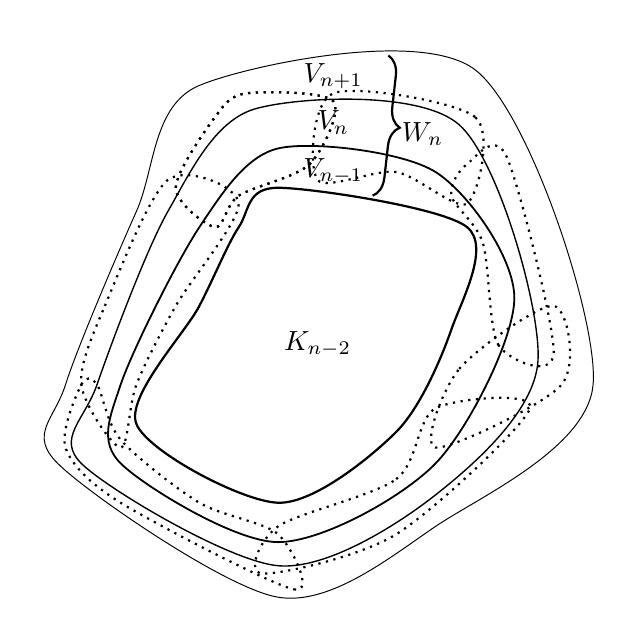
\begin{tikzpicture}
        \draw[line width=0.35] plot[smooth cycle] coordinates {
                (-0.8,1) (2,-0.7) (4,0.2) (6,2) (4.5,6) (1,5.8) (0.2,4.2) (-0.7,2)
            };
        \draw[line width=0.5] plot[smooth cycle] coordinates {
                (-0.5,1) (2,-0.3) (4,0.6) (5.3,2.3) (4.3,5.3) (1.7,5.5) (0.6,4.2) (-0.3,2)
            };
        \draw[line width=0.65] plot[smooth cycle] coordinates {
                (0,1) (2,0) (4,1) (5,3.1) (4,4.7) (2,5) (1,4) (0,2)
            };
        \draw[thick] plot[smooth cycle] coordinates {
                (0.2,1.5) (2,0.5) (3.5,1.4) (4.2,2.7) (4.4,4) (2,4.5) (1.5,4) (1,3)
            };
        \draw[thick, dotted] plot[smooth cycle] coordinates {
                (4.4,4.3) (4.5,5.4) (2.7,5.7) (2.5,4.6) (3.5,4.7)
            };
        \draw[thick, dotted] plot[smooth cycle] coordinates {
                (1.2,4) (0.7,4.5) (1.2,5.4) (1.6,5.7) (2.7,5.6) (2.4,4.8) (1.5,4.4)
            };
        \draw[thick, dotted] plot[smooth cycle] coordinates {
                (1.2,4) (0.7,4.5) (1.2,5.4) (1.6,5.7) (2.7,5.6) (2.4,4.8) (1.5,4.4)
            };
        \draw[thick, dotted] plot[smooth cycle] coordinates {
                (-0.5,2) (-0.2,3) (0.6,4.6) (1.5,4.3) (0.7,3) (0.2,2) (0,1.2)
            };
        \draw[thick, dotted] plot[smooth cycle] coordinates {
                (0,0.5) (2.2,-0.6) (2,0.1) (1,0.5) (0,1.3) (-0.3,2) (-0.5,2) (-0.7,1.2)
            };
        \draw[thick, dotted] plot[smooth cycle] coordinates {
                (2,0.2) (3.5,0.8) (4,1.7) (5.2,1.7) (3.5,0.1) (1.8,-0.4)
            };
        \draw[thick, dotted] plot[smooth cycle] coordinates {
                (4,1.2) (4.3,2.2) (5.5,3) (5.6,2)
            };
        \draw[thick, dotted] plot[smooth cycle] coordinates {
                (5.5,2.4) (4.8,2.5) (4.6,3.8) (4.2,4.4) (4.4,4.8) (4.9,4.9)
            };

        \node[anchor=north] at (2.5,2.8) {\(K_{n-2}\)};
        \node[anchor=north] at (2.7,5) {\(V_{n-1}\)};
        \node[anchor=north] at (2.7,5.6) {\(V_n\)};
        \node[anchor=north] at (2.7,6.2) {\(V_{n+1}\)};
        \draw[decorate,decoration={brace, amplitude=7pt}, thick] (3.4,6.18) -- (3.2,4.4) node[midway, yshift=-3pt, right=4pt] {\(W_n\)};
    \end{tikzpicture}
    \caption{The geometry of the finite subcover of \(V_n\subset W_n\) for some \(n\in\mathbb{N}\).}\label{fig:locallyfiniteopencoverexistence}
\end{figure}
\begin{remark}
    The property of local finiteness of an open collection \(S\) in \(\Omega\) is commonly stated as: for every \(z\in\Omega\), there exists an open neighborhood of \(z\) that intersects only finitely many sets in \(S\).

    This is equivalent to \cref{itm:locallyfiniteopencoverexistence_localfiniteness} in \cref{lem:locallyfiniteopencoverexistence}. Indeed, if every point has such a neighborhood, then any compact \(K\subset\Omega\) admits a finite subcover of these neighborhoods by Heine--Borel (\cref{thm:heineborel}), so \(K\) intersects finitely many sets in \(S\). Conversely, for any \(z\in\Omega\), take an open neighborhood \(V\ni z\) with relatively compact closure in \(\Omega\); then \(\overline{V}\) intersects finitely many sets in \(S\), and so does \(V\).
\end{remark}
\begin{theorem}[Partition of Unity]\label{thm:partitionofunity}
    Let \(\Omega\subseteq\mathbb{C}\) be a nonempty open set and let \(\cbraces{\Omega_k}_{k\in\mathbb{N}}\) be an open cover of \(\Omega\). Then there exists a collection of bump functions \(\cbraces{\alpha_j}_{j\in\mathbb{N}}\subset C^\infty(\mathbb{C})\), each with compact support in \(\Omega\), satisfying:
    \begin{enumerate}
        \item For each \(j\in\mathbb{N}\), there exists \(k\in\mathbb{N}\) such that \(\supp\qty(\alpha_j)\subseteq\Omega_k\).\label{itm:partitionofunity_subordinate}
        \item The collection \(\cbraces{\supp\qty(\alpha_j)}_{j\in\mathbb{N}}\) is locally finite.\label{itm:partitionofunity_localfiniteness}
        \item For each \(j\in\mathbb{N}\), \(0\le\alpha_j\le1\).\label{itm:partitionofunity_nonnegativity}
        \item \(\sum_{j=1}^\infty\alpha_j\equiv1\) on \(\Omega\).\label{itm:partitionofunity_partitionofunity}
    \end{enumerate}
    This is called a \(C^\infty\) partition of unity \textit{subordinate to} \(\cbraces{\Omega_k}_{k\in\mathbb{N}}\).
\end{theorem}
\begin{proof}
    For each \(z\in\Omega\) there exists \(r_z>0\) and \(k_z\in\mathbb{N}\) such that \(\overline{D\qty(z,r_z)}\subset\Omega_{k_z}\). The collection \(\cbraces{D(z,r)}{z\in\Omega\wedge0<r<r_z}\) is an open basis for \(\Omega\). By \cref{lem:locallyfiniteopencoverexistence} there exists a locally finite open cover \(\cbraces{D\qty(z_j,r_{z_j})}_{j\in\mathbb{N}}\subseteq\mathfrak{B}\) of \(\Omega\) with
    \[D\qty(z_j,r_{z_j})\subset\overline{D\qty(z_j,r_{z_j})}\subset\Omega_{k_{z_j}},\quad\forall j\in\mathbb{N}.\]
    Define the standard bump function
    \[\theta(z)=
        \begin{dcases}
            \exp\qty(\frac{1}{\abs{z}^2-1}) & \qif*\abs{z}<1,   \\
            0                               & \qif*\abs{z}\ge1.
        \end{dcases}\]
    For \(\varepsilon>0\) let \(\theta_\varepsilon(z)=\varepsilon^{-2}\theta\qty(\frac z\varepsilon)\), which has support \(\overline{D(0,\varepsilon)}\) and satisfies \[\int_{\mathbb{C}}\theta_\varepsilon(z)\ddx\wedge\ddy=1.\]
    Define \(\beta_j(z)=\theta_{r_{z_j}}\qty(z-z_j)\), so \(\supp(\beta_j)=\overline{D\qty(z_j,r_{z_j})}\subset\Omega_{k_{z_j}}\).

    By local finiteness of \(\cbraces{D\qty(z_j,r_{z_j})}_{j\in\mathbb{N}}\), for each \(z\in\Omega\) there exists an open neighborhood \(V\ni z\) intersecting only finitely many \(\overline{D\qty(z_j,r_{z_j})}\). Thus \(\cbraces{\supp(\beta_j)}_{j\in\mathbb{N}}\) is locally finite on \(\Omega\). Then the sum \(S(z)=\sum_{j=1}^\infty\beta_j(z)\) defined for \(z\in\Omega\) involves only finitely many nonzero terms (by local finiteness) on a neighborhood of every point \(z\). Hence \(S\in C^\infty(\Omega)\) and \(S(z)>0\) (since \(\cbraces{D\qty(z_j,r_{z_j})}_{j\in\mathbb{N}}\) covers \(\Omega\)). Define
    \[\alpha_j(z)=\frac{\beta_j(z)}{S(z)},\quad\forall j\in\mathbb{N}.\]
    Each \(\alpha_j\in C^\infty(\mathbb{C})\) has compact support in \(\Omega\), \(0\le\alpha_j\le1\), the supports are locally finite, and \(\sum_{j=1}^\infty\alpha_j(z)=1\) for all \(z\in\Omega\). Moreover \(\supp(\alpha_j)\subseteq\Omega_{k_{z_j}}\), proving subordination.
\end{proof}
\begin{theorem}[Existence of Bump Functions]\label{thm:bumpfunctionexistence}
    Let \(K\subset\mathbb{C}\) be compact and \(V\subset\mathbb{C}\) an open neighborhood of \(K\). Then there exists a compactly supported \(\varphi\in C^\infty(\mathbb{C})\) such that
    \[0\leq\varphi(z)\leq1\quad\forall z\in\mathbb{C},\]
    \(\supp(\varphi)\subset V\), and \(\varphi\equiv1\) on some open neighborhood of \(K\).
\end{theorem}
\begin{proof}
    Let \(V(K,\varepsilon)=\cbraces{z\in\mathbb{C}}{\inf_{\zeta\in K}\abs{z-\zeta}<\varepsilon}\) denote the open \(\varepsilon\)-neighborhood of \(K\). Since \(V\) is an open neighborhood of \(K\), \(\exists\varepsilon>0\) such that
    \[K\subset V(K,\varepsilon)\subset V(K, 2\varepsilon)\subset V,\]
    where \(A\subset\subset B\) means that the closure of \(A\) is compact and contained in \(B\).

    Define the open sets
    \[\Omega_1=V(K,2\varepsilon),\qquad\Omega_2=\mathbb{C}\setminus\overline{V(K,\varepsilon)}.\]
    Then \(\cbraces{\Omega_1,\Omega_2}\) is an open cover of \(\mathbb{C}\).

    By the Partition of Unity Theorem (\cref{thm:partitionofunity}), there exist compactly supported functions \(\cbraces{\alpha_j}_{j\in\mathbb{N}}\subset C^\infty(\mathbb{C})\) forming a partition of unity subordinate to this cover. That is,
    \[0\leq\alpha_j\leq1,\quad\supp\qty(\alpha_j)\subset\Omega_{i_j}\text{ for some }i_j\in\cbraces{1,2},\quad\sum_{j=1}^\infty\alpha_j\equiv1\qq{on}\mathbb{C}.\]
    Define
    \[\varphi(z)=\sum_{\substack{j\in\mathbb{N}\\\supp\qty(\alpha_j)\subset\Omega_1}}\alpha_j(z).\]
    Then \(\varphi\in C^\infty(\mathbb{C})\) is compactly supported within \(\Omega_1\), and since only finitely many \(\alpha_j\) are nonzero on a neighborhood of each point, \(\varphi\in C^\infty(\mathbb{C})\). Moreover, \(\supp(\varphi)\subset\Omega_1\subset V\).

    For \(z\in V(K,\varepsilon)\), all functions with support in \(\Omega_2\) vanish at \(z\), so
    \[\varphi(z)=\sum_{\supp\qty(\alpha_j)\subset\Omega_1}\alpha_j(z)=\sum_{j=1}^\infty\alpha_j(z)=1.\]
    Hence, \(\varphi\equiv 1\) on the open neighborhood \(V(K,\varepsilon)\) of \(K\). Outside \(V(K,2\varepsilon)\), all terms with support in \(\Omega_1\) vanish, so \(\varphi(z)=0\). Finally, \(0\leq\varphi\leq1\) everywhere by construction.

    Thus \(\varphi\) satisfies all required properties.
\end{proof}